\section{Progettazione Concettuale}
\subsection{Schema scheletro}
Un giocatore deve poter giocare a più partite contemporaneamente, quindi una semplice associazione tra giocatore e partita non è sufficiente ed è necessario avere un'entità PlayerInGame che contenga le informazioni del giocatore riguardanti una determinata partita. Inoltre, quest'ultima dovrà essere collegata con l'entità Color. Non potendo nella stessa partita avere più giocatori con lo stesso colore si è reso necessario evitare che esso fosse parte della chiave primaria del giocatore.

\begin{figure}[ht]
    \centering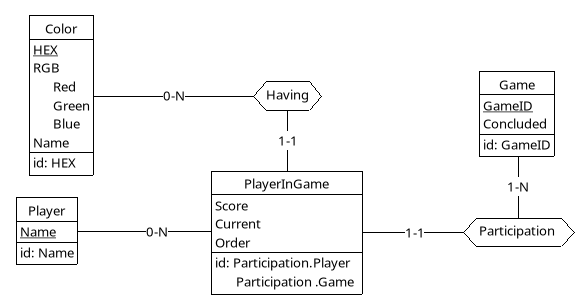
\includegraphics[scale=0.5]{images/Progettazione/Concettuale/Scheletro1.png}
    \caption{Schema scheletro riguandante giocatori, colori e game}
\end{figure}

Le entità Gameset, Tile e Meeple seguono un simile ragionamento riguardo al loro rapporto con una partita. Ognuna di queste entità ha un collegamento con il proprio "tipo": rispettivamente le entità GamesetType, TileType e MeepleType. Per tutti e tre viene fatta la distinzione tra le versioni presenti nel gioco base e quelle presenti nelle espansioni, è quindi chiaramente presente una generalizzazione che si divide in Basic (BasicGameset, BasicTile, BasicMeeple) e in Expansion (ExpansionGameset, ExpansionTile, ExpansionMeeple). Quest'ultima deve ovviamente essere connessa ad Expansion.
\clearpage

\begin{figure}[ht]
    \centering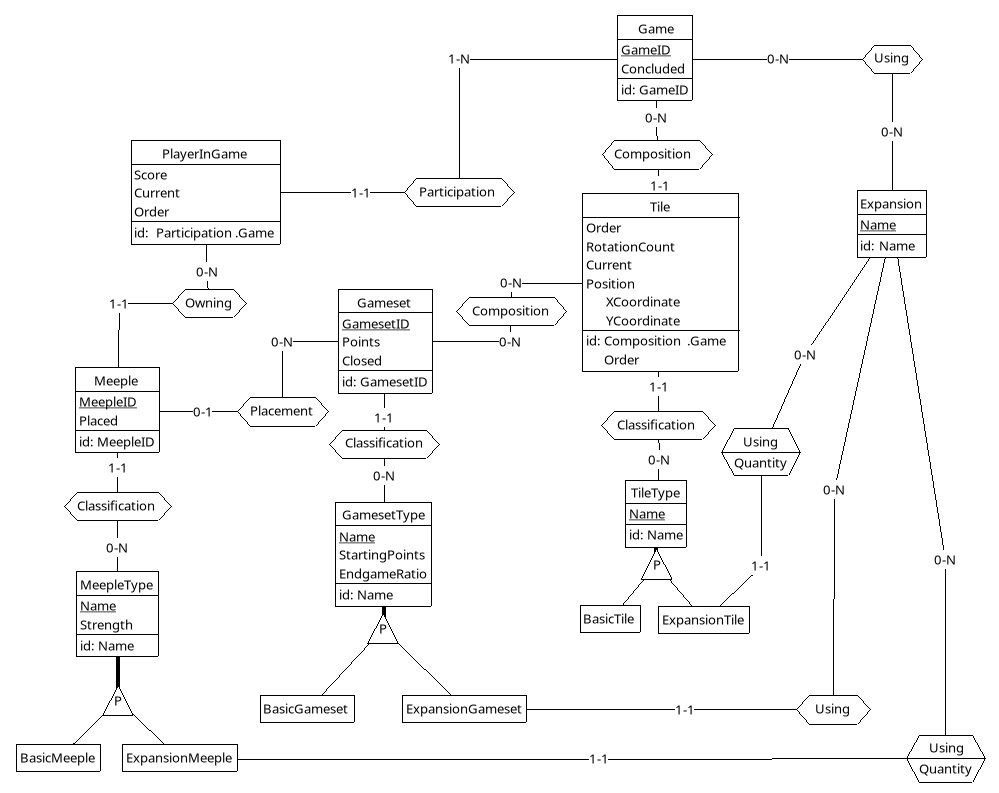
\includegraphics[scale=0.4]{images/Progettazione/Concettuale/Scheletro2.png}
    \caption{Schema scheletro riguandante strutture, tessere, meeple e espansioni}
\end{figure}

È necessario un modo per generare correttamente all'inizio della partita le Tile secondo il proprio tipo, a questo scopo si utilizza l'entità TileTypeConfiguration. Esso, per ogni TileType, contiene le informazioni riguardanti i tipi di sezione (entità TileSectionType) e i tipi di strutture (entità GamesetType) che dovranno essere presenti su tale tessera. Sulla base di GamesetType vengono poi creati Gameset che in combinazione con Tile e TileSectionType definiscono una TileSection. Su una TileSection può essere piazzato un Meeple e può essere ritenuta chiusa se combaciante con un'altra TileSection.
\clearpage

\begin{figure}[ht]
    \centering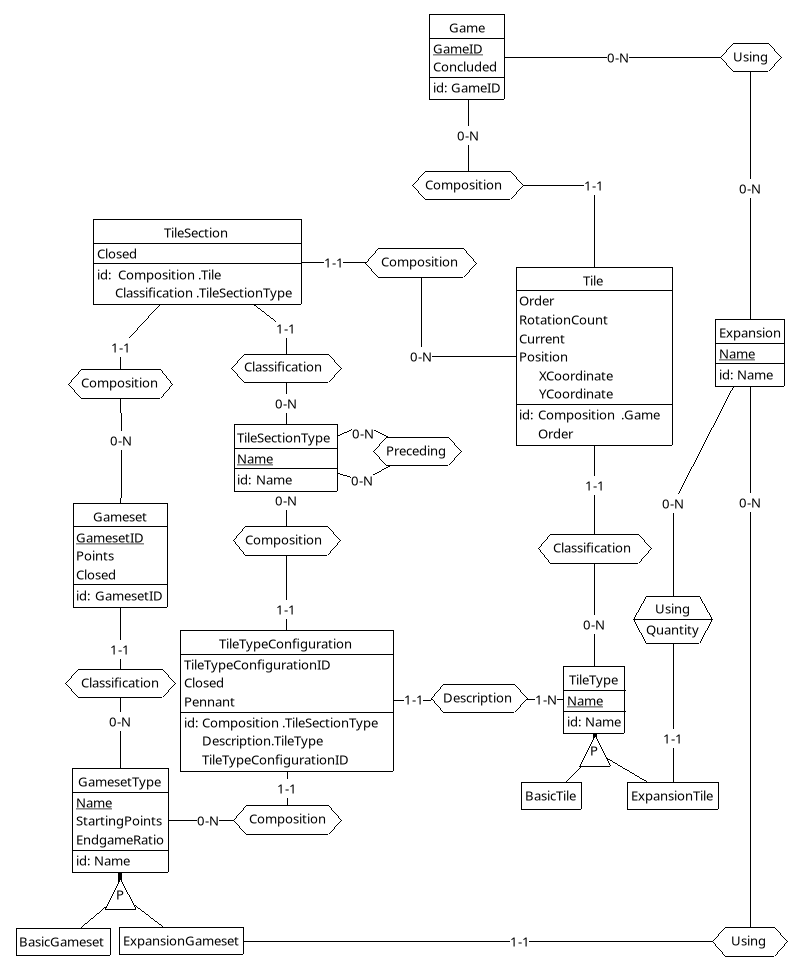
\includegraphics[scale=0.3]{images/Progettazione/Concettuale/Scheletro3.png}
    \caption{Schema scheletro riguandante la configurazione di tessere}
\end{figure}


Ogni partita deve essere ospitata all'interno di un Server e ogni Server deve far parte di una Region, che è a sua volta definita come la combinazione tra un Continent e un punto CardinalPoint.

\begin{figure}[ht]
    \centering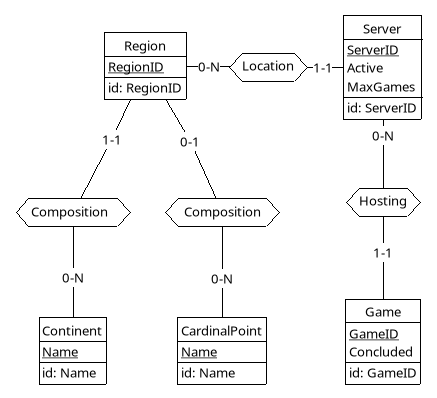
\includegraphics[scale=0.35]{images/Progettazione/Concettuale/Scheletro4.png}
    \caption{Schema scheletro riguandante la gestione dei server}
\end{figure}

\subsection{Schema concettuale finale}
\clearpage
\begin{figure}[ht]
    \centerline{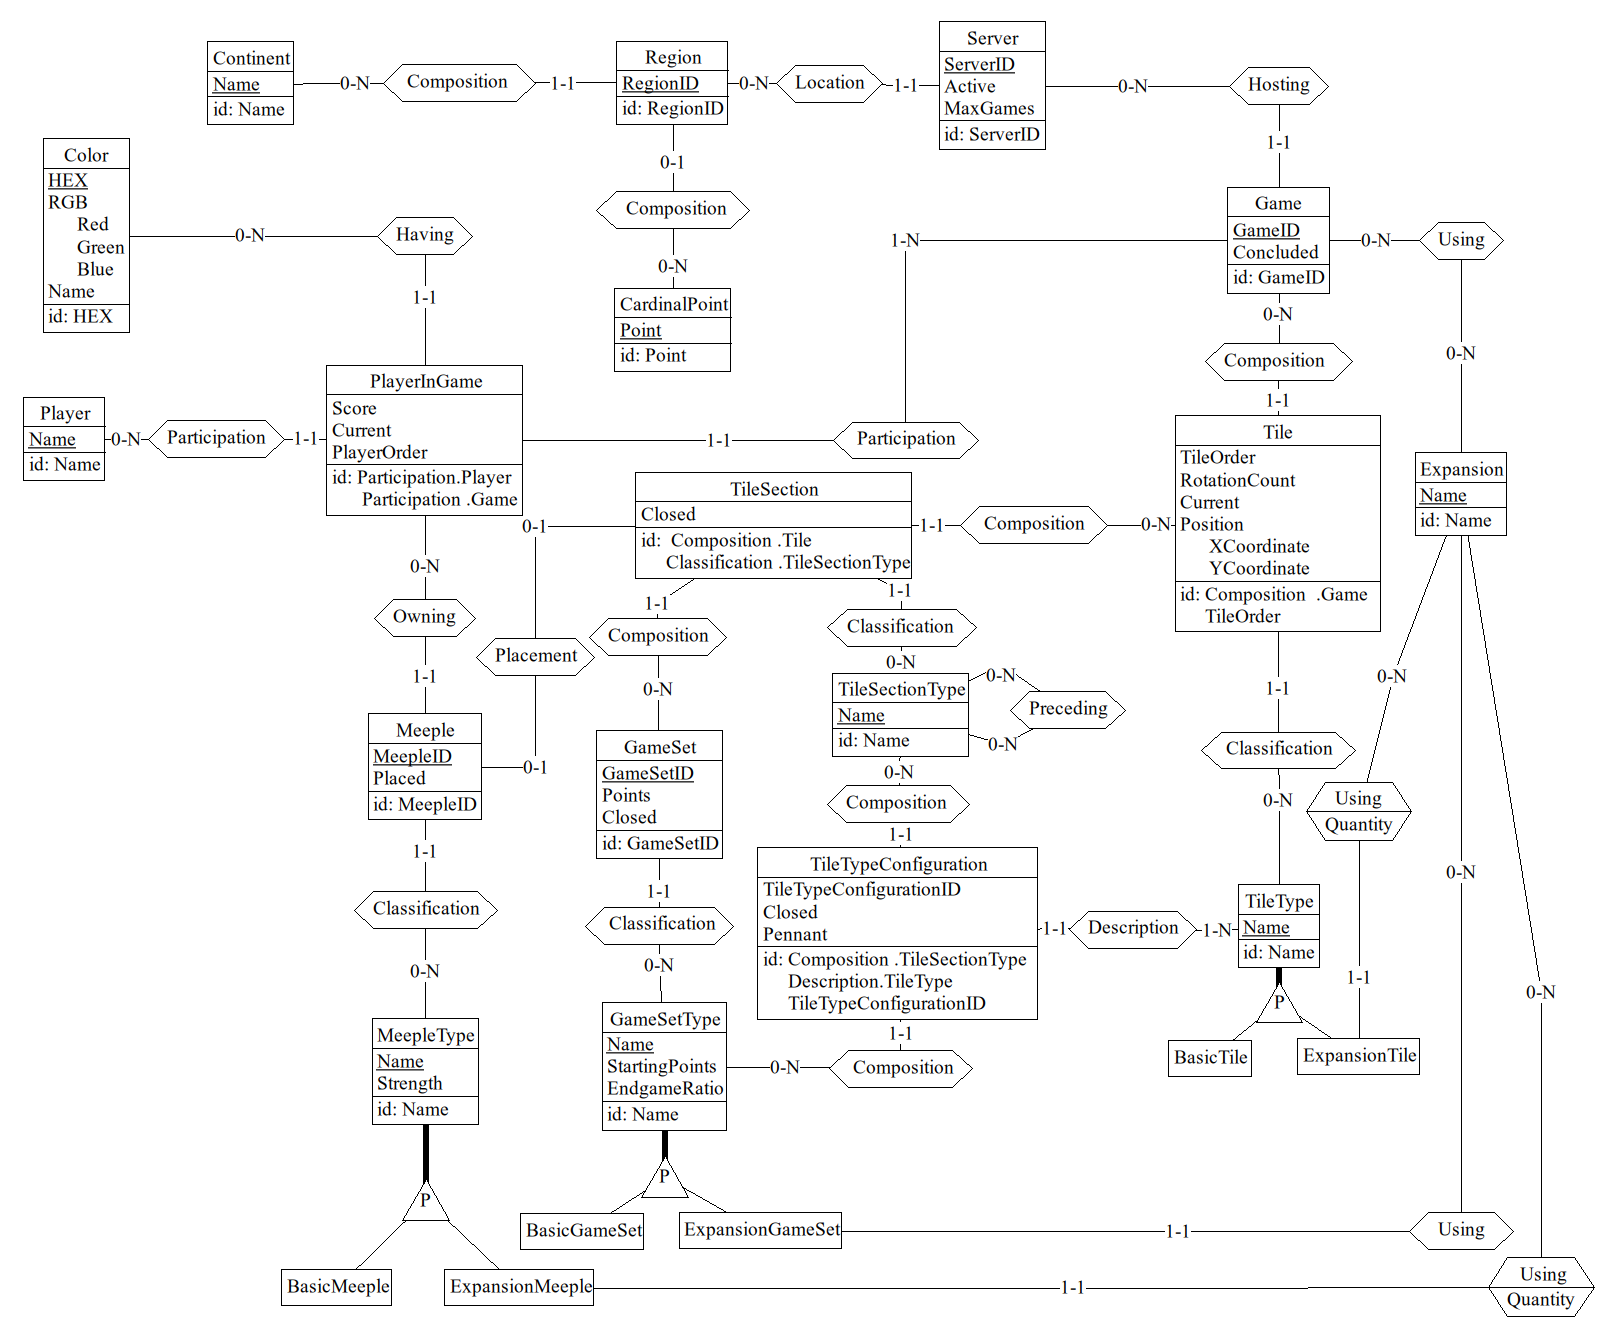
\includegraphics[scale=0.52]{images/Progettazione/Concettuale/modello.png}}
\end{figure}